\section{Deep Neural Networks}
In this section, we give a brief review of the deep learning architectures that we used
in network intrusion detection problem.

\subsection{Multilayer Perceptron}
Multilayer perceptron (MLP) is the simplest deep learning classifier in terms of
design of the architecture.
It is a fully connected feed-forward neural network, as shown in Figure~\ref{Fig:MLPArchitecture}.
By introducing non-linear neural units (perceptron), it can distinguish data that are
not linearly separable.
However, the non-linearity also make it very hard to train a deep MLP,
even if people have proposed the efficient back-propagation learning algorithm~\cite{Backpropagation}.
Recently it revived due to various new training techniques designed by deep learning community,
including Stochastic Gradient Descent (SGD),
batch normalization~\cite{BatchNorm} and Dropout~\cite{Dropout}.
Expect for the number of neurons in each layer and number of layers,
MPL can also be tuned with different activation functions.
The most popular ones are tangent, logistic and rectifier function.
\begin{figure}[h]
\centering
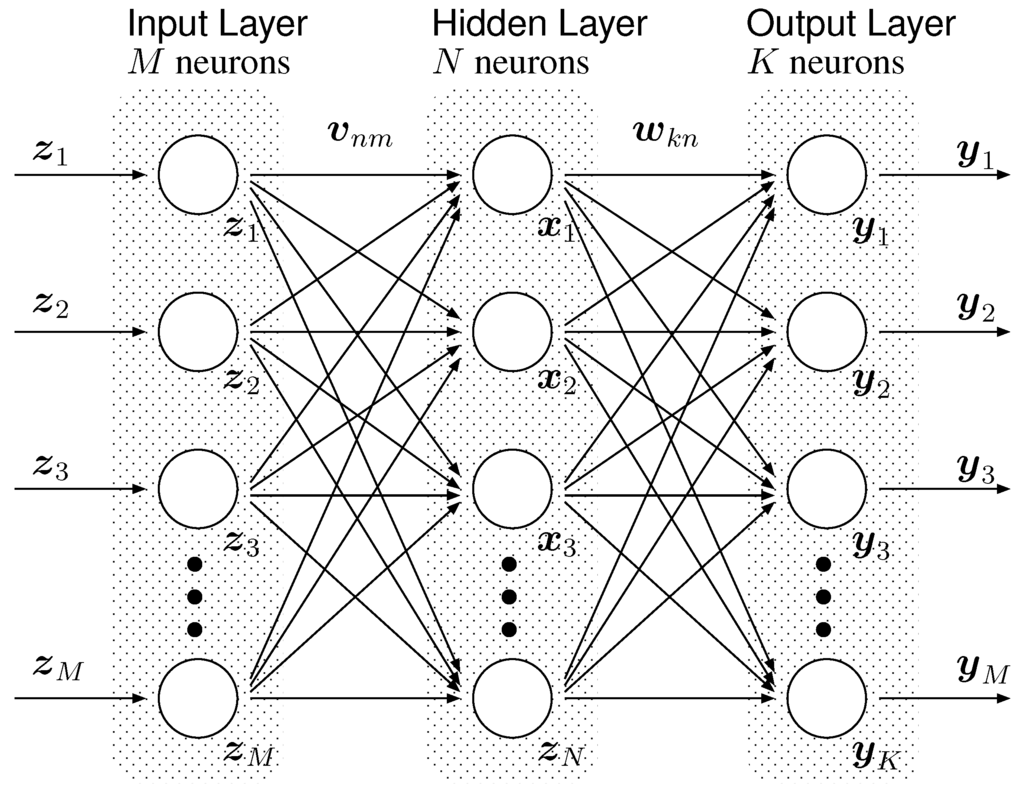
\includegraphics[width=0.45\textwidth]{figures/multilayer_perceptron.png}
\caption{A perceptron neural network with 1 hidden layer.
        Figure courtesy of Teijiro Isokawa, Haruhiko Nishimura and Nobuyuki Matsui.}
\label{Fig:MLPArchitecture}
\end{figure}

\subsection{Generative Models}
The amount of network traffic data is enormously large, usually in the order of terabytes
per day in a large monitored network.
This available big data makes deep learning techniques a promisingly better solution
to traffic classification.
In practice, however, the amount of data is impossible for a human security analyst to review,
e.g., to find patterns and label anomalies.
Generative model which can be trained unsupervisedly comes to rescue in that
\begin{itemize}
\item It utilizes the large amount of unlabeled data to learning useful and hierarchical features;
\item It is actually a way to initialize the weights in a deep neural network, which can be
        further fine-tuned to be a high performance classifier.
\end{itemize}
In this project we propose to try two generative models: restricted Boltzmann machine and autoencoders.


